\chapter{Aineisto}%
\label{ch:aineisto}

Työn toteuttamiseen käytettiin Cityscapes datasettiä \cite{Cordts2016Cityscapes}.


Datasetti pitää sisällään dispariteetti- sekä segmentaatiodatan.
Data on autosta stereokameralla kuvattua.
Malli on suunnattu automatisoituun liikenteeseen, ja se sisältää on paljon erilaisia kaupunkikuvia teiden varsilta.
Edellä mainittu tuottaa hankaluuksia lopputuloksen kanssa, koska malli toimii reaalimaailmassa vain kaupunkikuvissa,
mutta toisaalta parempaa disparteetti sekä segmentaatiomallia ei löytynyt. 
Tämän ongelman olisi voinut kiertää käyttämällä erillisiä malleja segmentointiin sekä dispariteettiin,
mutta kahden erialisen mallin yhdistäminen olisi tuonut enemmän riskejä.
Kahden mallin tapauksessa, jouduttaisiin joko luottamaan segmentaatiomalliin datan valmistelussa, 
tai kaikki data pitäisi käydä manuaalisesti läpi.

Data on kerätty erilaisista kaupunkiympäristöistä, ajoneuvon kyydistä kuvaten, ka tästä johtuen data on melko homogeenistä.
Dataan on merkattu monia erilaisia segmentoituja kohteita, kuten ihmisiä polkupyöriä ja autoja. 
Tämän työn kannalta tärkeintä on, että kaikki liikkuvat kohteet on merkattu.
Kaikki kuvat ovat stereo kuvia, sekä vasemmasta että oikeasta kamerasta kuvattuna.
Data on tämän työn kannalta melko helposti työstettävää, koska kuvat ovat ajoneuvosta otettuja ja kuvattava alue on näin ollen rajoittunut autolla ajettaviin alueisiin.
Tästä seuraa joitain rajoitteita datan käytössä, sillä mallin käyttö tämän datasetin ulkopuolisen datan kanssa ei ole kovin helppoa ilman uudelleenkouluttamista.
Kaupungit joista data on kerätty on enimmäkseen sakalaisia kaupunkeja.
Ne ovat kuvatuilla alueilla usein hyvin tiheään rakennettuja, josta syystä suurella osalla syvyyskartoista on selkeät reunat.

Jotta datasta saataisiin kattavampaa, olisi hyvä keskittyä muualta kuin kadulta kuvattuihin kuviin.
Tällöin lopullista mallia voisi yleistää toimimaan myös muissa kuin autoteiden tunnistamisessa.
Toinen parantamiskohde dataan voisi olla kuvaaminen kaupunkien ulkopuolelta,
jollaisia kuvia ei tästä datasetistä löydy johtuen kuvien alkuperäisestä käyttötarkoituksesta

\begin{figure}[h]
\centering
\pdftooltip{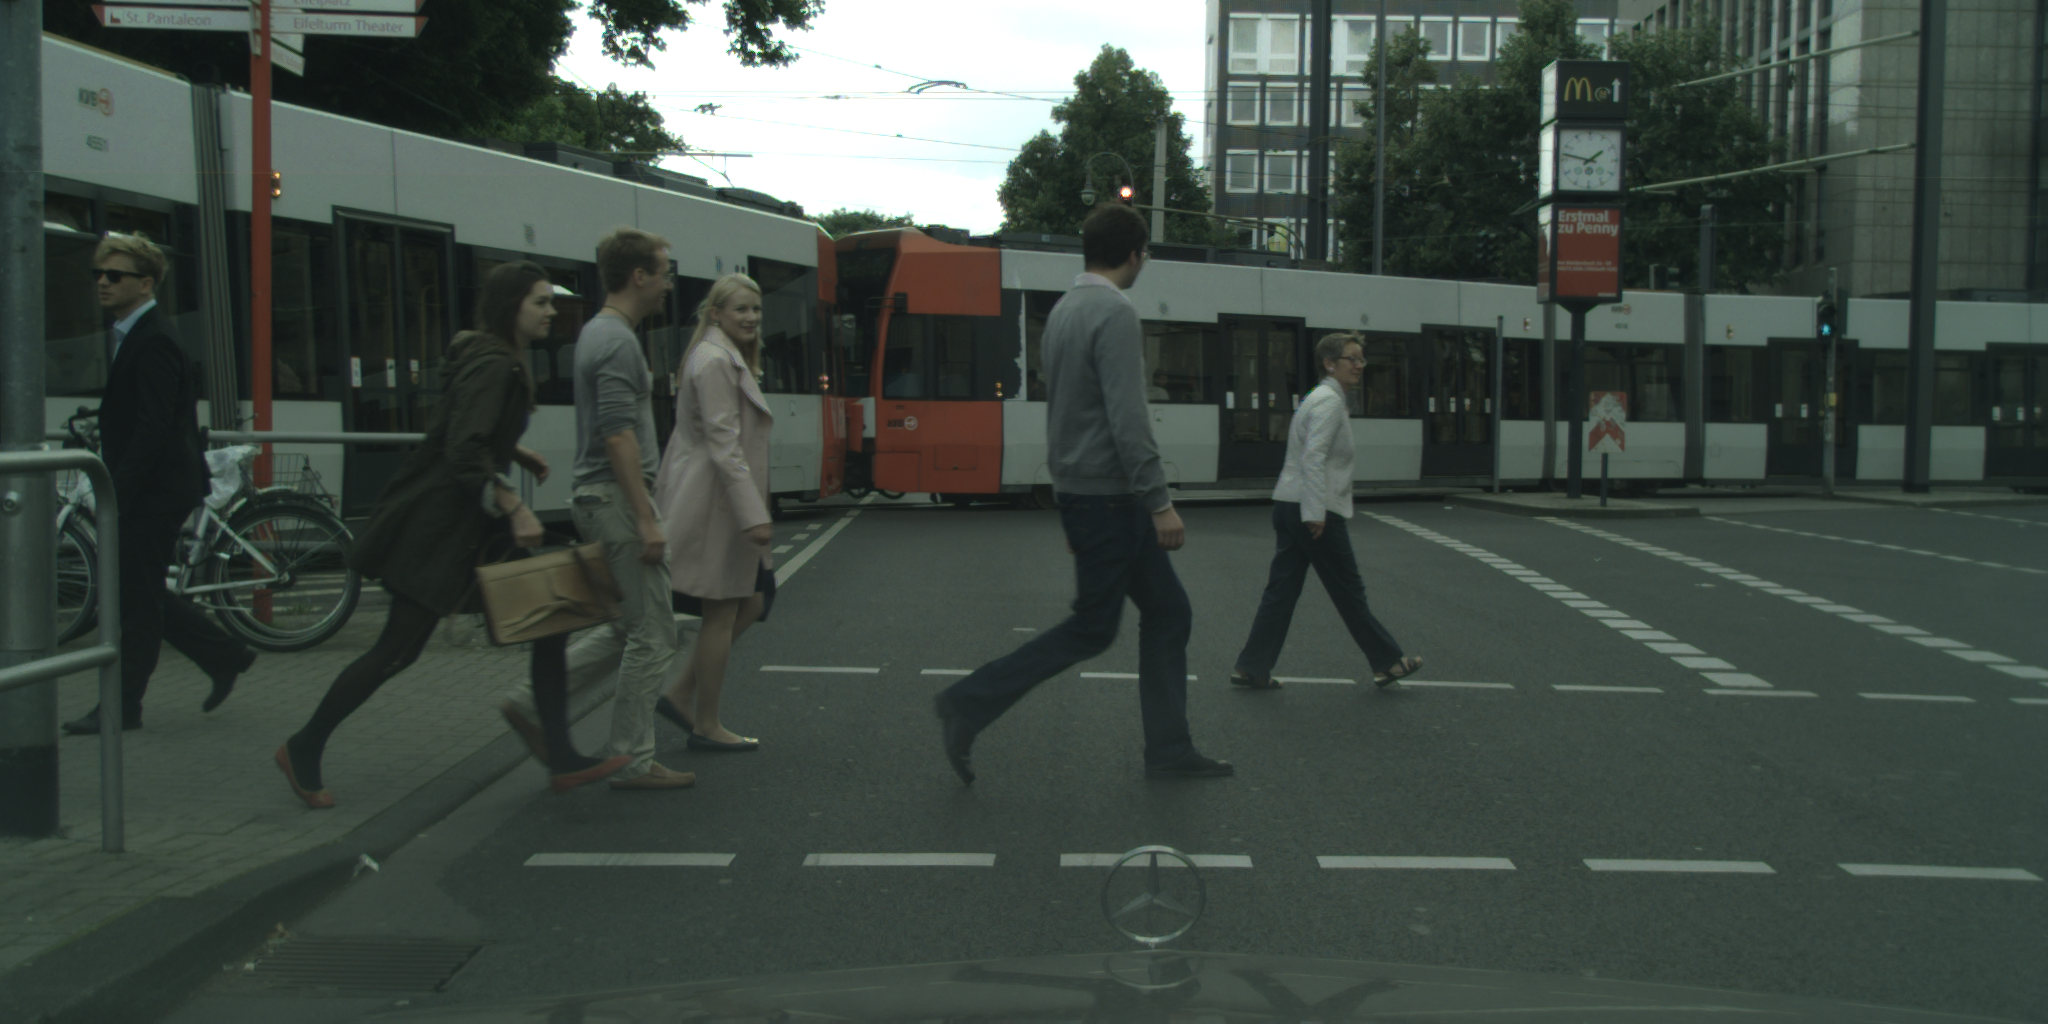
\includegraphics[width=\textwidth]{figures/extreme.png}}{extreme}
\caption{Esimerkki huonosta kuvasta}
\label{fig:extreme}
\end{figure}

    
Aineistossa on myös paljon tähän työhön soveltumattomia kuvia Kuva \ref{fig:extreme}.
Kuvassa on esimerkki tilanteesta jossa edes ihminen ei pysty ilman taustatietoa arvaamaan mitä liikkuvien kohteiden takana olisi.
Ilman jonkinlaista ulkoista tietoa ei tässä tapauksessa ole mahdollista tietää tilanteen totuutta.
Näin ollen vaihtoehdoksi jää totuuden generointi, mitä tässä työssä halutaan ratkaista,
vaikka lähtökohtaisesti paras lopputulos saadaankin oikealla datalla.
